\documentclass[11pt]{article}   	% use "amsart" instead of "article" for AMSLaTeX format

%\geometry{landscape}                		% Activate for rotated page geometry
%\usepackage[parfill]{parskip}    		% Activate to begin paragraphs with an empty line rather than an indent
%\usepackage{graphicx}				% Use pdf, png, jpg, or eps§ with pdflatex; use eps in DVI mode
								% TeX will automatically convert eps --> pdf in pdflatex		
\usepackage{amssymb}
\usepackage[cm]{fullpage}
\usepackage{tabularx}
\usepackage{float}
\usepackage{amsmath}
\usepackage{algorithmic}
\usepackage[hypcap]{caption}
\usepackage{graphicx}
\usepackage{framed}
\usepackage{subfigure}


%\floatstyle{boxed}
\restylefloat{figure}


%SetFonts

%SetFonts


\title{
	Machine Learning and Neural Computation\\
	\textbf{Assessed Coursework}
 }
\author{
	Beatriz Isabel Lopez Andrade (bil14)
}
%\date{}							% Activate to display a given date or no date

\begin{document}
\maketitle
\begin{abstract}
The present report assesses Monte-Carlo and Temporal Difference (specifically TD(0)) Reinforcement Learning methods for the Grid World discussed in the lecture notes. This report discusses the implementation and the influence of different parameters on the performance of both methods.
\end{abstract}

\section*{Introduction}
Unlike Dynamic Programming, Monte-Carlo and Temporal Difference methods do not need a complete knowledge of the environment[1], they can learn from experience, i.e. interactions with the environment. In the case of Monte-Carlo methods, this experience is a set of complete traces, from an initial state to an absorbing one, formed by several tuples (action, state, reward), that describe each of the transitions. Temporal Difference also uses traces, but it does not need complete ones, since it partially relies on previous estimations to perform policy evaluation, i.e. it bootstraps.

This report is divided into two sections, namely sections A and B. The first one focuses on Monte-Carlo Reinforcement Learning Methods. In particular, it discusses the implementation followed, First Visit Monte-Carlo, and the parameters that influence its performance. Section B 


[1] Reinforcement Learning

\section*{Section A}

This section briefly describes the implementation of \textbf{First-Visit Monte Carlo} and evaluates the performance of Monte-Carlo Reinforcement Learning method on GrindWorld1. In particular, it estimates the number of traces needed to compute an accurate state-action value function (Q) and the number of batches until the Optimal Policy is found. It also discusses the possible impact of other parameters, such as the discounted reward ($\gamma$) and the exploration-exploitation factor ($\epsilon$), on the previous computations.

In order to obtain the traces to perform Monte-Carlo and Temporal Difference estimations the function \texttt{GetTrace} is used. This function outputs a random episode from a given MDP. Each row in the output has three columns, that represent the reward for a transition from the previous state to the current one having taken a particular action, the current state, and the action taken in the current state to move to the following one.

In general, the function \texttt{GetTrace} generates a random sample of the current state taken into account the previous state and the chosen action in that state. After that, it gets the reward corresponding to that transition and action. If the current state is not an absorbing one, the function generates a random sample of the action in that state. On the contrary, if the current state is an absorbing one, none further actions are taken and therefore, the trace ends. The row corresponding to this state is formed by the reward, the state itself, and the action taken in the current state.

\begin{table}[!h] 
	\begin{center}
		\begin{tabular}{ | c c  c | }
		\hline
		Reward & Status & Action \\ \hline \hline
		0 & 4 & R \\ \hline
		-1 & 5 & R \\ \hline
		-1 & 6 & L \\ \hline
		1 & 5 & L \\ \hline
		1 & 4 & R \\ \hline
		-1 & 5 & R \\ \hline
		-1 & 6 & R \\ \hline
		10 & 7 & 0 \\ \hline
		\end{tabular}
		\caption{Trace corresponding to the Stair Climbing MDP.\label{tab:traceStair}}
		
	\end{center}
\end{table}

For the particular trace of \textbf{Stair Climbing MDP} in Table ~\ref{tab:traceStair}, the first state is four, because the function \texttt{StairClimbingMDP} assigns a probability of one to this state as the first state. The action in this state is \texttt{Right}, but it could have been \texttt{Left}, as the unbiased policy is used. In the following row, the state is five, since the probability of going from state four to five having taken action \texttt{Right} is one. The reward for this transition is -1 and the next action \texttt{Right}, but it could have been \texttt{Left}. The following rows are computed in the same way, until an absorbing state is reached.

In the case of the first row, there is no transition to get to the current state, i.e. it is the first state. Hence, there is no reward for getting to that particular state. That is the reason why a dummy value is assigned to the first reward.

In an absorbing state, the state where the trace ends, no further actions are taken. Therefore, the value for the last action is a dummy one.

The function \texttt{MonteCarloEstimation} implements \textbf{First-Visit Monte-Carlo} state-action value estimation. The signature of the function is the following:\\

\noindent\texttt{ [Q] = MonteCarloEstimation( T, R,  Initial, Absorbing, Policy, gamma, n)} \\
\\
\texttt{ T }$\equiv$ transition matrix,\\
\texttt{ R }$\equiv$ reward matrix,\\
\texttt{ Initial} $\equiv$ vector with the probabilities of being the first state for each non-absorbing state,\\
\texttt{ Absorbing} $\equiv$ vector whose values are 0 for non-absorbing states and 1 for absorbing ones,\\
\texttt{ Policy} $\equiv$ matrix with the probabilities of each action in each of the states,\\
\texttt{ gamma} $\equiv$ discounted reward,\\
\texttt{ n }$\equiv$ number of traces to sample.\\

The implementation of First-Visit Monte-Carlo is shown in procedural form in Figure~\ref{fig:mcfv}. The matrix of Q-values is estimated as the average of the returns following the first visit to state-action for all the traces.
\begin{figure}[!ht]
\begin{framed}
\begin{algorithmic}
 	\STATE SumReturns(s,a) $\leftarrow$ 0, $\forall$ s $\in$ States, $\forall$ a $\in$ Actions\;
 	\STATE N(s,a) $\leftarrow$ 0, $\forall$ s $\in$ States, $\forall$ a $\in$ Actions\;
	 \FOR{$i=1$ \TO n}
  		\STATE generate a new trace\;
  		\IF{first time (s,a) appearing in the trace}
   			\STATE R $\leftarrow$ return following the first occurrence of (s,a)\;
   			\STATE SumReturns(s,a) $\leftarrow$ SumReturns(s,a) + R\;
   			\STATE N(s,a) $\leftarrow$ N(s,a) + 1\;
  		\ENDIF
 	 \ENDFOR
 \STATE Q(s,a) $\leftarrow$ SumReturns(s,a) / N(s,a), $\forall$ s $\in$ States, $\forall$ a $\in$ Actions\;
\end{algorithmic}
\end{framed}
 \caption{First-Visit Monte-Carlo implementation.\label{fig:mcfv}}
 \end{figure}
 
The function \texttt{eGreedyPolicyFromQ} outputs an $\epsilon$-greedy policy based on the state-action value function. The signature of the function is the following:\\

\noindent\texttt{ [eGreedyPolicy] = eGreedyPolicyFromQ( T, Absorbing, epsilon)} \\
\\
\texttt{ T }$\equiv$ transition matrix,\\
\texttt{ Absorbing} $\equiv$ vector whose values are 0 for non-absorbing states and 1 for absorbing ones,\\
\texttt{ epsilon} $\equiv$ exploration-exploitation factor\\
 
The function \texttt{MonteCarloBatchOptimasation} implements on-policy Monte-Carlo Batch optimisation, where the Q and the $\epsilon$-greedy policy are updated in each batch, with the aim of converging to the optimal policy. The signature of the function is the following:\\

\noindent\texttt{ [eGreedyPolicy] = eGreedyPolicyFromQ( T, R,  Initial, Absorbing, Policy, gamma, epsilon, n, N)} \\
\\
\texttt{ T }$\equiv$ transition matrix,\\
\texttt{ R }$\equiv$ reward matrix,\\
\texttt{ Initial} $\equiv$ vector with the probabilities of being the first state for each non-absorbing state,\\
\texttt{ Absorbing} $\equiv$ vector whose values are 0 for non-absorbing states and 1 for absorbing ones,\\
\texttt{ Policy} $\equiv$ matrix with the probabilities of each action in each of the states,\\
\texttt{ gamma} $\equiv$ discounted reward,\\
\texttt{ epsilon} $\equiv$ exploration-exploitation factor\\
\texttt{ n }$\equiv$ number of traces per batch.\\
\texttt{ N }$\equiv$ number of batches.\\ 

These functions are used to compute the $\epsilon$-greedy policy on \texttt{GridWorld1} based on Monte-Carlo Reinforcement Learning. In order to obtain the policy from the state-action value function, the estimation of Q must be accurate. As the number of traces tends to infinity, the estimate of Q converges to its real value. In practice, however, the number of traces must be a finite value and, ideally, should be a small one. It is important to notice that this value not only depends on the complexity of the networks and the traces themselves, but also other parameters of the method, such as the discount factor $\gamma$, influence it.

The function \texttt{MonteCarloEstimationTestn} implements Monte-Carlo state-action value estimation (like \texttt{MonteCarloEstimation}) with on-line averaging. This function outputs the estimation of the state-action value function, the number of traces needed to converge with an accuracy level of 0.001 given a particular set of random traces, and the maximum value of the variance of the returns for each state and action. The number of traces needed to obtain an accurate estimation of Q and the maximum variance of the returns should be closely related: if the variance is high, the convergence is slow.

Figure~\ref{fig:maxvar} shows the mean of the maximum variance for 20 different state-action value function estimation (Q) and the corresponding mean of the number of sample traces needed to converge to an accurate estimation of Q for different values of the discount factor $\gamma$ (from 0.5 to 1). As stated before, when the variance is high, the number of traces needed to converge is also high; this is the case when $\gamma$=1, i.e. no \textit{discounting} is applied in the calculation of the return. The problem with this is that the sample traces can be arbitrarily long (they may include multiple loops). The return of traces with a high number of steps is prone to have a high absolute value, which may differ significantly from the returns of shorter traces; causing a high variance.\footnote{This values were computed assuming that S8 is the initial state.}

\begin{figure}
\centering
\setlength\fboxsep{0pt}
\setlength\fboxrule{0.5pt}
\fbox{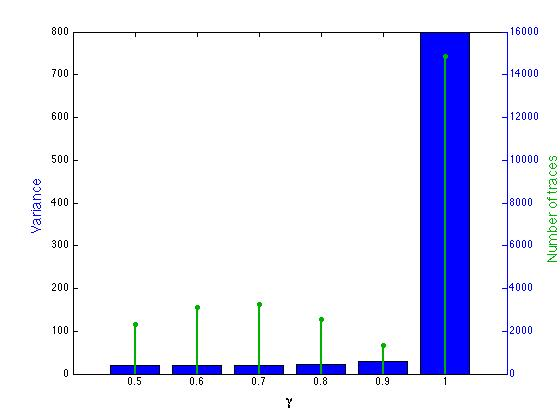
\includegraphics[scale=0.6]{./figures/fig_maximum_variance}}
\caption{Mean of the maximum variance of 20 different Q estimations and corresponding mean of the number of sample traces needed to converge to an accurate Q estimation for different values of $\gamma$. \label{fig:maxvar}}
\end{figure}

When $\gamma$ is low, the return maximizes immediate rewards. The problem with this is that actions taken to maximize returns in states "far" from the goal, may decrease the chances to get to the final goal, where the reward is high. This leads to the inability of computing optimal policies from the state-action value function. Figure~\ref{fig:gamma comp} shows the action with the highest probability in each state as computed by the function \texttt{MonteCarloBatchOptimasation} when $\epsilon=0.5$. For $\gamma$=0.5, the preferred actions in S9, S10, and S11 do not lead to S4 (absorbing state with the highest reward); this also happens in S9 when $\gamma$=0.6. For higher values of $\gamma$ \texttt{MonteCarloBatchOptimasation} converges to an Optimal Policy when the number of batches N is sufficiently large, assuming that the state-action value function estimates are accurate.

As the Figure~\ref{fig:maxvar} suggests, the mean number of sample traces needed to compute an estimation of Q with an accuracy level of 0.001 does not vary much for $\gamma$ between 0.5 and 0.9. Therefore, the value of the \textbf{discount factor $\gamma$} chosen is \textbf{0.9}, to ensure that the optimal actions have the highest probability in the $\epsilon$-greedy policy (obtained by calling the function \texttt{MonteCarloBatchOptimasation}).

\begin{figure}[ht!]
     \begin{center}
%
        \subfigure[Greedy Policy for $\gamma$=0.5]{%
            \label{fig:first}
            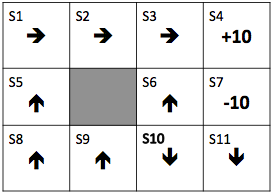
\includegraphics[scale=0.45]{./figures/gamma_05}
        }%
        \subfigure[Greedy Policy for $\gamma$=0.6]{%
           \label{fig:second}
           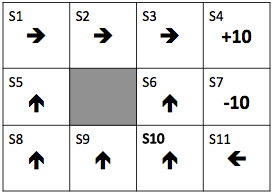
\includegraphics[scale=0.45]{./figures/gamma_06}
        }\\ %  ------- End of the first row ----------------------%
        \subfigure[Optimal Policy]{%
            \label{fig:third}
            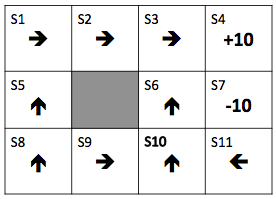
\includegraphics[scale=0.45]{./figures/optimal_policy}
        }%
        %
    \end{center}
    \caption{%
        Actions with the highest probabilities in the $\epsilon$-greedy policies computed using Monte-Carlo Batch optimization for $\gamma$ between 0.5 and 1, and $\epsilon=0.5$. 
     }%
   \label{fig:gammacomp}
\end{figure}


\subsection*{Question 2}

In the case of \texttt{GridWorld1}, the number of traces needed to get an accurate estimation of the state-value function is about 16250. With this number of traces, the maximum difference between the values of the state-value function between two consecutive iterations is less than 0.001, and therefore, convergence is assumed. The number of batches needed until converge to the optimal policy is 5.



\end{document}  